\documentclass{article}

\usepackage{tikz}
\usepackage{caption}


\begin{document}

\title{Sparse Matrix-Vector Multiplication with CUDA}
\author{Georgii Evtushenko}

\maketitle

\begin{abstract}
Standard methods of differential equations discretization usually lead to systems of linear equations. 
A general feature of produced systems is that the number of entries in each equation depends on local topological features of the discretization.
Thus, the matrices generated by these systems contain a lot of zeroes. It's possible to take advantage of knowledge about zeroes' position by 
storing matrices in special data structures.The abstract data type for these structures is called the sparse matrix. 
This post provides an efficiency review for basic sparse matrix data structures.
\end{abstract}

\section{Introduction}
Here is the text of your introduction.

\begin{figure}
  \centering
  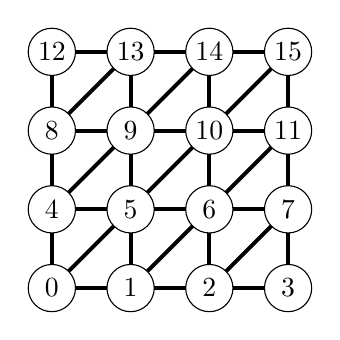
\begin{tikzpicture}[circ/.style = {circle, draw, inner sep=0pt, minimum size=3pt, outer sep=0pt, minimum size=6mm}]
    \foreach \x in {0,...,3}
    {
      \foreach \y in {0,...,3}
      {
        \pgfmathtruncatemacro{\label}{\y * 4 + \x}
        \node (\x\y) [circ] at (\x, \y) {\label};
      }
    }

    \foreach \x in {1,...,3}
    {
      \foreach \y in {0,...,3}
      {
        \pgfmathtruncatemacro{\px}{\x - 1}
        \draw [line width=0.5mm] (\x\y) -- (\px\y);
      }
    }

    \foreach \x in {0,...,3}
    {
      \foreach \y in {1,...,3}
      {
        \pgfmathtruncatemacro{\py}{\y - 1}
        \draw [line width=0.5mm] (\x\y) -- (\x\py);
      }
    }

    \foreach \x in {1,...,3}
    {
      \foreach \y in {1,...,3}
      {
        \pgfmathtruncatemacro{\py}{\y - 1}
        \pgfmathtruncatemacro{\px}{\x - 1}
        \draw [line width=0.5mm] (\x\y) -- (\px\py);
      }
    }
  \end{tikzpicture}
  \caption{A simple finite element mesh model}
\end{figure}

\section{Data Structures for Sparse Matrices}
Write your subsection text here.

\subsection{COO}

\subsection{CSR}

\subsection{ELL}

\subsection{Hybrid}

\subsection{DIA}


\section{Conclusion}
Write your conclusion here.

\end{document}
